\chapter {Алгоритми за графи}

\section{Обхождане на граф}

\subsection{Обхождане в дълбочина}

\subsection{Обхождане в широчина}

\begin{itemize}
\item
  
\item 
  Алгоритъмът работи както за ориентирани, така и за неориентирани графи.
\end{itemize}

\section{Минимално покриващо дърво на граф}

\begin{itemize}
\item
  Един граф $G = (V,E)$ се нарича {\bf свързан}, ако има път между всеки два $v,v^\prime \in V$.
\item 
  Един граф $G$ се нарича {\bf дърво}, ако $G$ е свързан неориентиран граф без цикли.
\item
  {\bf Покриващо дърво} за свъзан неориентиран граф $G = (V,E)$,
  е дърво $T = (V,E^\prime)$, $Е^\prime \subseteq E$.
\item
  {\bf Минимално покриващо дърво} свъзан неориентиран граф $G = (V,E,c)$
  е покриващо дърво $T$, за което числото $r = \sum_{e\in T} c(e)$ е минимално.
\end{itemize}

\subsection{Алгоритъм на Прим}

Нека е даден неориентиран свързан претеглен граф $G = (V,E,c)$
и да фиксираме един връх $r \in V$, който ще бъден корен покриващото дърво.

\begin{enumerate}
\item 
  Започваме от дървото $T_0 = (\{r\},\emptyset)$.
\item
  Нека сме построили дървото $T_i = (V_i,E_i)$.
  Търси реброто $(v,v^\prime)$ с минимално тегло, за което
  $v \in V_i$ и $v^\prime \in V \setminus V_i$.
  Образуваме \[T_{i+1} = (V_i\cup\{v^\prime\}, E_i \cup \{(v,v^\prime)\}).\]
\item
  Алгоритъмът завършва когато $V_i = V$.
\end{enumerate}

\subsection{Алгоритъм на Крускал}

Нека е даден неориентиран свързан претеглен граф $G = (V,E,c)$.
\begin{enumerate}
\item
  Нека $V = \{v_0,\dots,v_n\}$.
  Строим редица от дървета $\{T_i\}_{i \leq n}$, като
  $T_i = (\{v_i\},\emptyset)$, т.е. дърветата са съставени само от един връх и нямат ребра.
  Ще се стремим да обединяваме тези дървете и най-накрая да получим само едно дърво.
\item
  Сортираме ребрата $E$ на графа $G$ във възходящ ред относно тяхната цена.
\item
  За всяко ребро $(v,v^\prime) \in E$, нека $v$ принадлежи на върховете на $T$, а $v^\prime$ 
  принадлежи на върховете на $T^\prime$.
  \begin{itemize}
  \item 
    Ако $T \neq T^\prime$, то обединяваме $T$ и $T^\prime$ като добавяме към техните ребра $(v,v^\prime)$.
    Така получаваме с единица по-къса редица от дървета.
  \item
    Ако $T = T^\prime$, то не правим нищо.    
  \end{itemize}  
\item
  Алгоритъмът завършва или когато сме обходили всички ребра, или
  когато сме получили редица от дървета с дължина 1.
\end{enumerate}

\section{Минимални пътища от даден връх}

\begin{itemize}
\item
  С $u \stackrel{p}{\leadsto} v$ означаваме, че $p$ е път от $u$ до $v$.
\item
  Тук ще разглеждаме ориентирани графи $G = (V,E)$, като имаме и 
  функция $w: E\to \R$, която задава {\bf тегла} на ребрата на графа.
\item 
  {\bf Цена на път} $p = (v_0,\dots,v_k)$ в графа означаваме 
  \[w(p) = \sum_{i<k} w(v_i,v_{i+1}).\]
\item
  За всеки два върха $u,v \in V$, означаваме
  \begin{align*}
    \delta(u,v) = 
    \begin{cases}
      \min\{w(p)\mid u \stackrel{p}{\leadsto} v\}, \mbox{ ако има път от }u\mbox{ до }v\\
      \infty, \mbox{ иначе }
    \end{cases}
  \end{align*}
\item
  {\bf Минимален път} $p$ от $u$ до $v$ е такъв път, за който $w(p) = \delta(u,v)$.
\item
  Имаме следното важно свойство.
  Нека $u \stackrel{p}{\leadsto} v$ и $p$ е {\bf минимален път}.
  Да означим $p = (v_0,\dots,v_k)$ и $p_{ij} = (v_i,\dots,v_j)$ за $0\leq i \leq j \leq k$.
  Тогава за всеки $0\leq i \leq j \leq k$, 
  $p_{ij}$ е {\bf минимален път} от $v_i$ до $v_j$.
\item
  {\bf Цикъл} е път $p = (v_0,\dots,v_k)$, където $v_0 = v_k$.
\item
  Също така казваме, че по пътя $p = (v_0,\dots,v_k)$ има цикъл, ако
  за някои $0 \leq i < j \leq k$ имаме, че $v_i = v_j$.
\item
  Ако има цикъл с отрицателно тегло по някой път от $u$ до $v$, то 
  тогава пишем, че $\delta(u,v) = -\infty$.
\item
  Нека $u \stackrel{p}{\leadsto} v$ и $p$ е с минимално тегло.
  Тогава няма цикъл с положително тегло по $p$.
\item
  Нека $u \stackrel{p}{\leadsto} v$ и $p$ е с минимално тегло.
  Можем без ограничение на общността да приемем, че няма цикли с нулево тегло
  по $p$.
\item
  Важно свойство е, че броят на върховете по всички минални пътища е $\leq \abs{V}$.
\end{itemize}

\begin{prop}
  Нека $u \stackrel{p}{\leadsto} v$, където $p$ е с минимално тегло.
  Тогава няма цикъл с положително тегло по $p$.
\end{prop}
\begin{proof}
  Нека $p = (v_0,\dots,v_k)$, $v_0 = u$, $v_k = v$ и 
  $c = (v_i,\dots,v_j)$, за някои $0 \leq i < j \leq k$, 
  като $w(c) > 0$. Щом $c$ е цикъл, то $v_i = v_j$.
  Но тогава пътя $p^\prime = (v_0,\dots,v_i,v_{j+1},\dots,v_k)$ също е път от $u$ до $v$.
  Освен това, $w(p^\prime) = w(p) - w(c) < w(p)$.
  Получихме, че пътя $p^\prime$ има по-малко тегло от пътя $p$.
  Това е противоречие с минималността на теглото на пътя $p$.
\end{proof}




Нека да фиксираме един връх $s \in V$.
Нашата цел е да намерим минимални пътища от $s$ до всички достижими от $s$ върхове,
както и тяхната цена. 
Да отбележим, че ако имаме отрицателен по някой път $s \leadsto v$, то задачата не е добре 
дефинирана, защото тогава $\delta(s,v) = -\infty$.

За тази цел въвеждаме два масива, $dist$ и $pred$, с дължина $\abs{V}$.
\begin{itemize}
\item 
  $dist[v]$ - дава цена на минимален път от $s$ до $v$.
  Ако $dist[v] = \infty$, то не е намерен път $s\leadsto v$.
\item
  $pred[v]$ - дава предшественика на $v$ по този минимален път, т.е.
  ако $pred[v] = u$, то $s \leadsto u \to v$.
  Ако $pred[v] = NIL$, то не е намерен път $s \leadsto v$.
\item
  Сега като имаме масива $pred$, можем да образуваме графа на предшествениците $G_{pred} = (V_{pred},E_{pred})$, където
  \begin{enumerate}[]
  \item 
    $V_{pred} = \{u \in V \mid pred[u] \neq NIL \} \cup \{s\}$,
  \item
    $E_{pred} = \{(u,v) \in V\times V \mid pred[v] = u\}$.
  \end{enumerate}
\end{itemize}

% \begin{figure}[!ht]
%   \centering
% \begin{subfigure}{0.5\textwidth}
%   \centering
% % \begin{algorithm}
%   % \caption{INIT(s)}
%   % \label{alg:init}
%   \begin{algorithmic}[1]
%     \FORALL{$v \in V$}
%     \STATE $dist[v] := \infty$
%     \STATE $pred[v] := NIL$
%     \ENDFOR
%     \STATE $dist[s] := 0$
%   \end{algorithmic}
% % \end{algorithm}
% \end{subfigure}
% \hfill
% \begin{subfigure}{0.5\textwidth}
%   \centering
% % \begin{algorithm}
%   % \caption{UPDATE(u,v)}
%   % \label{alg:update}
%   \begin{algorithmic}[1]
%     \IF{$dist[v] > dist[u] + w(u,v)$}
%     \STATE $dist[v] := dist[u] + w(u,v)$
%     \STATE $pred[v] := u$
%     \ENDIF
%   \end{algorithmic}
% % \end{algorithm}
% \end{subfigure}
% \end{figure}

\begin{algorithm}
  \caption{INIT(s)}
  \label{alg:init}
  \begin{algorithmic}[1]
    \FORALL{$v \in V$}
    \STATE $dist[v] := \infty$
    \STATE $pred[v] := NIL$
    \ENDFOR
    \STATE $dist[s] := 0$
  \end{algorithmic}
\end{algorithm}

\begin{algorithm}
  \caption{UPDATE(u,v)}
  \label{alg:update}
  \begin{algorithmic}[1]
    \IF{$dist[v] > dist[u] + w(u,v)$}
    \STATE $dist[v] := dist[u] + w(u,v)$
    \STATE $pred[v] := u$
    \ENDIF
  \end{algorithmic}
\end{algorithm}

\subsection{Основни свойства}
  
\begin{prop}[Неравенство на триъгълника]
  \label{prop:triangle}
  За всяко $(u,v) \in E$,
  \[\delta(s,v) \leq \delta(s,u) + w(u,v).\]
\end{prop}

\begin{prop}
  \label{prop:upper-bound}
  Нека сме изпълнили INIT(s).
  Тогава имаме свойството \[(\forall v\in V)[dist[v] \geq \delta(s,v)].\]
  То се запазва и след прозволен брой изпълнения на UPDATE върху ребра на графа.
  
  Освен това, ако веднъж $dist[v] = \delta(s,v)$, то $dist[v]$
  повече не се променя.
\end{prop}
\begin{proof}
  Индукция по броя $i$ на изпълнения на UPDATE.
  За $i = 0$ е очевидно.
  Ще докажем твърдението за $i > 0$ изпълнения на UPDATE.
  Нека $dist[v] > dist[u] + w(u,v)$ и изпълним UPDATE(u,v).
  Тогава като използваме индукционното предположение и неравенството на триъгълника,
  \begin{align*}
    dist[v] & = dist[u] + w(u,v)\\
    & \geq \delta(s,u) + w(u,v)\\
    & \geq  \delta(s,v).
  \end{align*}

  Ясно е, че веднъж достигнали $dist[v] = \delta(s,v)$, $dist[v]$
  не може да се промени, защото тази стойност може само да намалява, а ние
  сме достигнали нейния минумум.
\end{proof}

\begin{prop}
  \label{prop:no-path}
  Нека сме изпълнили INIT(s)
  и нека няма път от $s$ до $v$.
  Тогава имаме свойството
  \[dist[v] = \delta(s,v) = \infty.\]
  То се запазва и след прозволен брой изпълнения на UPDATE върху ребра на графа.
\end{prop}
\begin{proof}
  Щом няма път от $s$ до $v$, то $\delta(s,v) = \infty$.
  От Твърдение \ref{prop:upper-bound}, $dist[v] \geq \delta(s,v) = \infty$.
  Следователно, $dist[v] = \infty$.
\end{proof}

% \begin{proof}
%   Индукция по броя на изпълнения $i$ на UPDATE.
  
%   За $i = 0$, то твърдението е очевидно.
%   Да приемем, че то е вярно за $\leq i$.
%   Нека $(i+1)$-то изпълнение е UPDATE(u,v), за някое $u \in V$,
%   само в този случай можем да променим стойността на $v$.
  
%   Ако $dist[u] = \infty$, то $dist[v] = dist[u] + w(u,v)$ и нищо не правим.
%   Ако $dist[u] < \infty$, то това означава, че има път от $s$ до $u$, 
%   защото от твърдение ...., $\infty > dist[u] \geq \delta(s,u)$.
%   \begin{itemize}
%   \item 
%     ако има ребро $(u,v) \in E$, то това означава, че има път $s \leadsto u \to v$,
%     което е противоречие с условието.
%   \item
%     ако няма ребро $(u,v)\not\in E$, $w(u,v) = \infty$ и $dist[v] = \infty$.
%   \end{itemize}
% \end{proof}


% \begin{prop}
%   Нека $(u,v) \in E$.
%   Тогава веднага след изпълнението на UPDATE(u,v) имаме, че
%   \[dist[v] \leq dist[u] + w(u,v).\]
% \end{prop}


\begin{prop}
  \label{prop:converge}
  Нека $s\leadsto u \to v$ е път с минимално тегло.
  Нека сме изпълнили INIT(s) и няколко на брой UPDATE, като измежду тях и UPDATE(u,v).
  Ако по някое време преди изпълнение на UPDATE(u,v) 
  имаме, че $dist[u] = \delta(s,u)$, то след това изпълнение
  $dist[v] = \delta(s,v)$ и повече не се променя.
\end{prop}
\begin{proof}
  Първо да отбележим, че за $(u,v) \in E$, веднага след изпълнението на UPDATE(u,v) имаме, че
  \[dist[v] \leq dist[u] + w(u,v).\]
  Ако $dist[u] = \delta(s,u)$, то от Твърдение \ref{prop:upper-bound} това равенство се запазва.
  Получаваме, че:
  \begin{align*}
    dist[v] & \leq dist[u] + w(u,v)\\
    & = \delta(s,u) + w(u,v)\\
    & = \delta(s,v),
  \end{align*}
  защото $s\leadsto u \to v$ е път с минимална дължина.
  Тогава $dist[v] \leq \delta(s,v)$ и следователно 
  \[dist[v] = \delta(s,v),\]
  защото пак от Твърдение \ref{prop:upper-bound}, винаги е изпълнено, че $dist[v] \geq \delta(s,v)$,
\end{proof}

\begin{prop}
  \label{prop:path-update}
  Да разгледаме пътя $p = (v_0,\dots,v_k)$, като $v_0 = s$.
  Нека сме изпълнили INIT(s) и след това няколко пъти UPDATE, като сме включили 
  UPDATE($v_{i}$,$v_{i+1}$), за всяко $0\leq i < k$, в този ред на изпълнение.
  Тогава най-накрая получаваме, че $dist[v_k] = \delta(s,v_k)$.
\end{prop}
\begin{proof}
  Индукция по $i$.
  В началото, $dist[v_0] = dist[s] = 0 = \delta(s,s)$.
  Ако $dist[v_{i-1}] = \delta(s,v_{i-1})$, то след изпълнение на UPDATE($v_{i-1}$,$v_{i}$),
  получаваме от Твърдение \ref{prop:converge}, че $dist[v_i] = \delta(s,v_{i})$.
\end{proof}

\begin{prop}
  \label{prop:tree-shortest-path}
  Нека сега да приемем, че в нашия граф няма цикли с отрицателни тегла, достижими от $s$
  и нека сме изпълнили INIT(s) и произволен брой пъти UPDATE.
  Тогава:
  \begin{enumerate}[1)]
  \item 
    $G_{pred}$ е дърво с корен $s$.
  \item
    ако $(\forall v\in V)[dist[v] = \delta(s,v)]$, то $G_{pred}$ е дърво на пътищата с минимални тегла с корен $s$.
  \end{enumerate}
\end{prop}
\begin{proof}
  \begin{enumerate}[1)]
  \item 
    Първо ще докажем, че $G_{pred}$ е насочен ацикличен граф и след
    това, че няма пътища $p \neq p^\prime$ от вида $s\stackrel{p}{\leadsto} v$ и $s\stackrel{p^\prime}{\leadsto} v$.
    \begin{itemize}
    \item 
      Да допуснем, че $G_{pred}$ е цикличен граф.
      Нека $c = (v_0,\dots,v_k)$ е цикъл, $v_0 = v_k$, който се е получил точно след изпълнение на 
      UPDATE($v_{k-1}$,$v_k$).

      Да разгледаме ситуацията преди изпълнението на UPDATE($v_{k-1}$,$v_{k}$).
      Имаме, че 
      \[(\forall i < k)[pred[v_{i+1}] = v_{i}]\]
      от което следва, че
      \[(\forall i < k-1)[dist[v_{i+1}] \geq dist[v_i] + w(v_i,v_{i+1})].\]
      Щом още нямаме цикъл, преди изпълнението на UPDATE($v_{k-1}$,$v_k$) имаме, че
      \[dist[v_{k}] > dist[v_{k-1}] + w(v_{k-1},v_k).\]
      Получаваме, че
      \begin{align*}
        \sum^{k}_{i = 1} dist[v_{i}] & > \sum^{k-1}_{i=0} (dist[v_i] + w(v_{i},v_{i+1}))\\
        & = \sum^{k-1}_{i=0} dist[v_i] + w(c),
      \end{align*}
      но понеже $v_0 = v_k$, 
      \[\sum^{k-1}_{i=0} dist[v_i] = \sum^{k}_{i=1} dist[v_i]\]
      и тогава
      \[0 > w(c).\]
      Получаваме, че цикълът $c$ има отрицателно тегло, което е противоречие.
    \item
      Да допуснем, че има $p \neq p^\prime$  и  $s\stackrel{p}{\leadsto} v$ и $s\stackrel{p^\prime}{\leadsto} v$.
      Това означава, че съществуват $x \neq y$,
      $s \leadsto u \leadsto x \to z \leadsto v$ и $s \leadsto u \leadsto y \to z \leadsto v$.
      По определение, $pred(z) = x \neq y = pred(z)$. Противоречие.
    \end{itemize}
  \item
    \begin{itemize}
    \item 
      Лесно се съобразява, че $V_{pred}$ съдържа точно върховете достижими от $s$,
      защото $v$ е достижим от $s$ точно когато $\delta(s,v) = dist[v] < \infty$, 
      но тогава $pred[v] \neq NIL$.
    \item
      Вече доказахме в 1), че $G_{pred}$ е дърво с корен $s$.
    \item
      Остана да докажем, че ако имаме $s\stackrel{p}{\leadsto} v$ в $G_{pred}$, 
      то $p$ е път с минимално тегло в $G$.
      Нека $p = (v_0,\dots,v_k)$, $v_0 = s$, $v_k = v$.
      По условие, 
      \[(\forall i < k)[dist[v_i] = \delta(s,v_i)],\]
      а от факта, че $(\forall i < k)[pred[v_i] = v_{i-1}]$ следва, че
      \[(\forall i < k)[dist[v_i] \geq dist[v_{i-1}] + w(v_{i-1},v_{i})].\]
      Като обединим горните две неравенства, получваме, че
      \[(\forall i < k)[w(v_{i-1},v_{i}) \leq \delta(s,v_{i}) - \delta(s,v_{i-1})],\]
      Тогава
      \begin{align*}
        w(p) & = \sum^k_{i=1} w(v_{i-1},v_{i})\\
        & \leq \sum^k_{i=1} (\delta(s,v_i)- \delta(s,v_{i-1}))\\
        & = \delta(s,v_k) - \delta(s,v_0)\\
        & = \delta(s,v_k) - \delta(s,s)\\
        & = \delta(s,v_k) - 0\\
        & = \delta(s,v_k).
      \end{align*}
      Следователно, 
      \[w(p) \leq \delta(s,v_k).\]
      Понеже $\delta(s,v_k)$ е минималното тегло на път от $s$ до $v_k$,
      то $w(p) = \delta(s,v_k)$.
      Следователно, $p$ е път с минимално тегло.
    \end{itemize}
  \end{enumerate}
\end{proof}




\subsection{Алгоритъм на Дейкстра}
\index{Дейкстра!алгоритъм}

В този алгоритъм, разглеждаме ориентирани графи $G = (V,E,c)$ с {\em положителни} тегла (или цени) по ребрата, т.е. 
имаме функция $c:E\to\R^+$. 
Целта на алгоритъма е да построим следните функции:
\begin{itemize}
\item 
  $\delta: V\to\R\cup\{\infty\}$, 
  която да дава минималната цена на път от $s$ до $v$. Ако няма път от $s$ до $v$, то $\delta(v)$
  ще приема стойност $\infty$.
\item
  $\pi:V\to V\cup\{\infty\}$, която да дава предшественика на $v$ по път с минимална цена от $s$ до $v$,
  ако такъв път съществува, иначе ще дава като резултат $\infty$.
\end{itemize}

\begin{algorithm}
\caption{Алгоритъм на Дейкстра}
\label{alg:dijkstra}

\begin{algorithmic}[1]
  \REQUIRE{$w:E\to \R^+$}
  \STATE INIT(s)
  \STATE $V^\prime := V$
  \WHILE{$V^\prime\neq\emptyset$}
  % \AND $(\exists u\in V^\prime)[dist[u] < \infty]$}
  \STATE Избираме $u_0\in V^\prime$, за който $ dist[u_0] = min\{dist[v] \mid v\in V^\prime\} $
  \STATE $V^\prime := V^\prime\setminus\{u_0\}$
  \FORALL{ $v\in V^\prime $ }
  \IF{$(u_0,v)\in E$}
  \STATE UPDATE($u_0$,$v$)
    % \AND $\delta(v) > \delta(u_0) + c(u_0,v)$}
  % \STATE $\delta(v):= \delta(u_0)+c(u_0,v)$
  % \STATE $\pi(v) := u_0$
  \ENDIF
  \ENDFOR
  \ENDWHILE
  % \RETURN $\delta$
\end{algorithmic}
\end{algorithm}

\begin{thm}
  Нека $G$ е ориентиран граф с неотрицателни тегла по ребрата.
  След изпълнението на алгоритъма на Дейкстра с начален връх $s$,
  \[(\forall v \in V)[dist[v] = \delta(s,v)].\]
\end{thm}
\begin{proof}
  Ще докажем, че на всяка итерация на while-цикъла, 
  \[(\forall v\in V\setminus V^\prime)[dist[v] = \delta(s,v)].\]
  Първоначално $V\setminus V^\prime = \emptyset$.
  Ще докажем, че на всяка итерация на while-цикъла, за върха $u$, който сме премахнали от $V^\prime$,
  е изпълнено, че $dist[u] = \delta(s,u)$.
  За целта да допуснем противното и нека $u$ е първия връх, който е премахнат от $V^\prime$,
  за който $dist[u] \neq \delta(s,u)$.
  Лесно се съобразява, че $u \neq s$.
  Освен това, трябва $s \leadsto u$, защото иначе $dist[u] = \delta(s,u) = \infty$ според Твърдение \ref{prop:no-path}.
  Нека $s \stackrel{p}{\leadsto} u$ и $p$ е път с минимално тегло.
  Да разбием пътя $p$ по следния начин:
  \[s \stackrel{p_1}{\leadsto}x\to y\stackrel{p_2}{\leadsto}u,\]
  където $y$ е първия връх по пътя $p$, за който $y\not\in V^\prime$.
  Ясно е, че тогава $x \in V^\prime$ и тогава $dist[x] = \delta(s,x)$, 
  защото ние избрахме $u$ да бъде първия връх, за който $dist[u] \neq \delta(s,u)$.
  На итерацията на while-цикъла, на която добавяме $x$ към $V^\prime$, 
  ние изпълняваме UPDATE(x,y) и според Твърдение \ref{prop:converge}, $dist[y] = \delta(s,y)$.
  Но понеже $y$ е преди $u$ по път с минимално тегло и при положение, че няма ребра с отрицателни тегла,
  \[\delta(s,y) \leq \delta(s,u).\]
  Тогава
  \begin{align*}
    dist[y] & = \delta(s,y) \\
    & \leq \delta(s,u)\\
    & \leq dist[u], \mbox{според Твърдение \ref{prop:upper-bound}}.
  \end{align*}
  Но понеже $y,v \not\in V^\prime$ и сме избрали $u$ вместо $y$, то това означава, че
  \[dist[u] \leq dist[y].\]
  Следователно, 
  \[dist[y] = dist[u]\]
  и тогава 
  \[dist[u] = \delta(s,u),\]
  с което достигаме до противоречие.
\end{proof}
\begin{cor}
  $G_{pred}$ е дърво на минималните пътища с корен $s$.
\end{cor}


Ако във $V^\prime$ има останали върхове $v$, то те имат $\delta(v) = \infty$, т.е.
те са недостижими от $s$ и следователно пътят от $s$ до $v$ има дължина $\infty$.

Фигура \ref{fig:dijkstra-table} илюстрира как се променя функцията $\delta$ по време на изпълнението на алгоритъма.
Освен това, с лека модификация на горния алгоритъм, можем да намерим не само стойността на най-късите пътища, но
и списък с ребрата, които участват във всеки от тях. Фигура \ref{fig:dijkstra-graph} илюстрира това.
Ребрата, оцветени в зелено, са тези, които участват в най-късите пътища.
Жълти ребра са тези, които са кандидати да участват в най-късите пътища.
Червени са тези ребра, които са били вече обходени и са отхвърлени като част от най-къс път.

\tikzstyle{weight} = [font=\small]
\tikzstyle{value} = [font=\small]
\tikzstyle{edge} = [draw,thick,-]
\tikzstyle{nodedecorate}=[shape=circle,draw,thick,font=\small]
\tikzstyle{arrowdecorate}=[->,>=stealth,thick]

% Rename: selected --> current
\tikzstyle{selected vertex}=[vertex, fill=yellow!50]
\tikzstyle{selected edge} = [draw,line width=5pt,-,yellow!50]

\tikzstyle{vertex}=[circle,minimum size=15pt,inner sep=0pt]
\tikzstyle{sure vertex} = [vertex, fill=green!30]

\tikzstyle{path edge} = [draw,line width=5pt,-,red!50]

\tikzstyle{sure edge} = [draw,line width=5pt,-,green!30]
% \tikzstyle{ignored edge} = [draw,line width=5pt,-,black!20]


\begin{figure}[!htbp]
  \begin{subfigure}[b]{0.5\textwidth}
    \begin{tikzpicture}[]
      
      \foreach \nodename/\x/\y/\direction/\navigate in { a/1/1/above/north,
        b/0/0/left/west, c/1/-1.5/below/south, d/3/1/above/north, e/3/-1.5/below/south, f/5/0.5/right/east, g/5/2.5/right/east}
      {
        \node (\nodename) at (\x,\y) [nodedecorate] {};
        \node [\direction] at (\nodename.\navigate) {$\nodename$};
      }
      %% edges or lines
      \path
      \foreach \startnode/\endnode/\direction/\weight in {b/a/above/7,
        b/c/below/2, c/a/left/4, a/d/below/4, c/e/below/5, d/c/left/8, e/d/right/3}
      {
        (\startnode) edge[arrowdecorate] node[\direction] {$\weight$} (\endnode)
      }
      
      \foreach \startnode/\endnode/\direction/\angle/\weight in {
        a/g/above/15/10, d/f/above/15/5, d/g/above/-15/2, f/d/below/15/1, g/f/right/15/6, e/f/below/-15/7}
      {
        (\startnode) edge[arrowdecorate,bend left=\angle] node[\direction] {$\weight$} (\endnode)
      };
    \end{tikzpicture}
    \caption{Пример за насочен граф с тегла по ребрата}
  \end{subfigure}
 \quad
 \begin{subtable}[b]{0.5\textwidth}
   \begin{tabular}[b]{|c|c|c|c|c|c|c|c|c|}
     \hline
     $\delta(a)$ & $\delta(b)$ & $\delta(c)$ & $\delta(d)$ & $\delta(e)$ & $\delta(f)$ & $\delta(g)$\\
     \hline
     $\infty$ & {\bf \framebox{0}} & $\infty$ & $\infty$ & $\infty$ & $\infty$ & $\infty$ \\
     \hline
     7 & $\colon$ & {\bf \framebox{2}} & $\infty$ & $\infty$ & $\infty$ & $\infty$ \\
     \hline
      {\bf \framebox{6}} & $\colon$ & $\colon$ & $\infty$ & 7 & $\infty$ & $\infty$ \\
      \hline
      $\colon$ & $\colon$ & $\colon$ & 10 & {\bf \framebox{7}} & $\infty$ & 16 \\
      \hline
      $\colon$ & $\colon$ & $\colon$ & {\bf \framebox{10}} & $\colon$ & 14 & {\bf 12} \\
      \hline
      $\colon$ & $\colon$ & $\colon$ & $\colon$ & $\colon$ & 14 & {\bf \framebox{12}} \\
      \hline
      $\colon$ & $\colon$ & $\colon$ & $\colon$ & $\colon$ & {\bf \framebox{14}} & $\colon$ \\
      \hline
      $\colon$ & $\colon$ & $\colon$ & $\colon$ & $\colon$ & $\colon$ & $\colon$ \\
      \hline
    \end{tabular}
    \caption{Разстояния с начален връх $b$}
  \end{subtable}
  \caption{Алгоритъм на Дейкстра}
  \label{fig:dijkstra-table}
\end{figure}


\begin{figure}[!htbp]
  \index{Дейкстра!алгоритъм}
  

\subfigure[Започваме от съседите на $a$]{
  \begin{tikzpicture}[scale=0.9]
    % nodes
    \foreach \nodename/\x/\y/\value/\direction/\navigate/\color in { 
      a/0/0/0/above/north/green, 
      b/-1/1/\infty/left/west/black, 
      c/2.5/1/\infty/above/north/black, 
      d/2/-0.5/\infty/below/south/black,
      e/-1/-0.5/\infty/below/south/black, 
      f/0.5/2/\infty/above/north/black,
      g/0/-1.8/\infty/below/south/black, 
      h/2.5/-1.8/\infty/right/east/black}
    {
        \node[vertex, nodedecorate, fill=\color!25] (\nodename) at (\x,\y) {$\value$};
        \node [\direction] at (\nodename.\navigate) {$\nodename$};
      };
      % edges
      \path
      \foreach \startnode/\endnode/\direction/\angle/\weight in {
        e/b/left/15/5, e/g/below/-15/3, d/g/below/15/2, 
        g/a/left/15/2, a/g/right/30/9, f/c/below/-15/1,
        c/f/above/-30/5, c/h/right/15/2, c/d/above/-15/1,
        f/d/left/-15/4, a/b/below/0/2, b/f/above/0/1, 
        a/d/above/0/8}
      {
        (\startnode) edge[arrowdecorate,bend left=\angle] node[\direction] {$\weight$} (\endnode)
      };
    \end{tikzpicture}
  }
  \subfigure[$b$ е най-близко до $a$]{
    \begin{tikzpicture}[scale=0.9]
      %nodes
      \foreach \nodename/\x/\y/\value/\direction/\navigate/\color in { 
        a/0/0/0/above/north/green, 
        b/-1/1/2/left/west/yellow, 
        c/2.5/1/\infty/above/north/black, 
        d/2/-0.5/8/below/south/yellow,
        e/-1/-0.5/\infty/below/south/black, 
        f/0.5/2/\infty/above/north/black, 
        g/0/-1.8/9/below/south/yellow, 
        h/2.5/-1.8/\infty/right/east/black}
      {
        \node[vertex, nodedecorate, fill=\color!25] (\nodename) at (\x,\y) {$\value$};
        \node [\direction] at (\nodename.\navigate) {$\nodename$};
      };

      \path
      \foreach \startnode/\endnode/\direction/\angle in {
        a/g/right/30, a/b/above/0, a/d/above/0}
      {
        (\startnode) edge[selected edge,bend left=\angle] node[\direction] {} (\endnode)
      };
      %edges
      \path
      \foreach \startnode/\endnode/\direction/\angle/\weight in {
        e/b/left/15/5, e/g/below/-15/3, d/g/below/15/2, g/a/left/15/2, a/g/right/30/9, f/c/below/-15/1, c/f/above/-30/5,
        c/h/right/15/2, c/d/above/-15/1, f/d/left/-15/4, a/b/below/0/2, b/f/above/0/1,  a/d/above/0/8}
      {
        (\startnode) edge[arrowdecorate,bend left=\angle] node[\direction] {$\weight$} (\endnode)
      };
    \end{tikzpicture}
  }
  \subfigure[Най-къс път до $f$]{
    \begin{tikzpicture}[scale=0.9]
      %nodes
      \foreach \nodename/\x/\y/\value/\direction/\navigate/\color in { 
        a/0/0/0/above/north/green, 
        b/-1/1/2/left/west/green,
        c/2.5/1/\infty/above/north/black, 
        d/2/-0.5/8/below/south/yellow,
        e/-1/-0.5/\infty/below/south/black, 
        f/0.5/2/3/above/north/yellow, 
        g/0/-1.8/9/below/south/yellow, 
        h/2.5/-1.8/\infty/right/east/black}
      {
        \node[vertex, nodedecorate, fill=\color!25] (\nodename) at (\x,\y) {$\value$};
        \node [\direction] at (\nodename.\navigate) {$\nodename$};
      };
      \path
      (a) edge[sure edge] node[] {} (b);
      \path
      \foreach \startnode/\endnode/\direction/\angle in {
        a/g/right/30, a/d/above/0}
      {
        (\startnode) edge[selected edge,bend left=\angle] node[\direction] {} (\endnode)
      };
      \path
      \foreach \startnode/\endnode/\direction/\angle in {
         b/f/above/0}
      {
        (\startnode) edge[selected edge, bend left=\angle] node[\direction] {} (\endnode)
      };
      %edges
      \path
      \foreach \startnode/\endnode/\direction/\angle/\weight in {
        e/b/left/15/5, e/g/below/-15/3, d/g/below/15/2, g/a/left/15/2, a/g/right/30/9, f/c/below/-15/1, c/f/above/-30/5,
        c/h/right/15/2, c/d/above/-15/1, f/d/left/-15/4, a/b/below/0/2, b/f/above/0/1,  a/d/above/0/8}
      {
        (\startnode) edge[arrowdecorate,bend left=\angle] node[\direction] {$\weight$} (\endnode)
      };
    \end{tikzpicture}
  }
  \subfigure[По-къс път до $d$ и $c$]{
    \begin{tikzpicture}[scale=0.9]
      % nodes
      \foreach \nodename/\x/\y/\value/\direction/\navigate/\color in { 
        a/0/0/0/above/north/green,
        b/-1/1/2/left/west/green,
        c/2.5/1/4/above/north/yellow, 
        d/2/-0.5/7/below/south/yellow,
        e/-1/-0.5/\infty/below/south/black, 
        f/0.5/2/3/above/north/green, 
        g/0/-1.8/9/below/south/yellow, 
        h/2.5/-1.8/\infty/right/east/black}
      {
        \node[vertex, nodedecorate, fill=\color!25] (\nodename) at (\x,\y) {$\value$};
        \node [\direction] at (\nodename.\navigate) {$\nodename$};
      };
      \path
      (a) edge[sure edge] node[] {} (b)
      (b) edge[sure edge] node[] {} (f);
      
      \path
      \foreach \startnode/\endnode/\direction/\angle in {
        a/d/above/0}
      {
        (\startnode) edge[path edge,bend left=\angle] node[\direction] {} (\endnode)
      };
      \path
      \foreach \startnode/\endnode/\direction/\angle in {f/c/below/-15/1, f/d/left/-15/4, a/g/right/30}
      {
        (\startnode) edge[selected edge, bend left=\angle] node[\direction] {} (\endnode)
      };
      %edges
      \path
      \foreach \startnode/\endnode/\direction/\angle/\weight in {
        e/b/left/15/5, e/g/below/-15/3, d/g/below/15/2, g/a/left/15/2, a/g/right/30/9, f/c/below/-15/1, c/f/above/-30/5,
        c/h/right/15/2, c/d/above/-15/1, f/d/left/-15/4, a/b/below/0/2, b/f/above/0/1,  a/d/above/0/8}
      {
        (\startnode) edge[arrowdecorate,bend left=\angle] node[\direction] {$\weight$} (\endnode)
      };
    \end{tikzpicture}
  }
  \subfigure[По-къс път до $d$ и $h$]{
    \begin{tikzpicture}[scale=0.9]
      % nodes
      \foreach \nodename/\x/\y/\value/\direction/\navigate/\color in { 
        a/0/0/0/above/north/green,
        b/-1/1/2/left/west/green,
        c/2.5/1/4/above/north/green,
        d/2/-0.5/5/below/south/yellow,
        e/-1/-0.5/\infty/below/south/black, 
        f/0.5/2/3/above/north/green, 
        g/0/-1.8/9/below/south/yellow, 
        h/2.5/-1.8/6/right/east/yellow}
      {
        \node[vertex, nodedecorate, fill=\color!25] (\nodename) at (\x,\y) {$\value$};
        \node [\direction] at (\nodename.\navigate) {$\nodename$};
      };
      \path
      (a) edge[sure edge] node[] {} (b)
      (b) edge[sure edge] node[] {} (f)
      (f) edge[sure edge, bend left=-15] node[] {} (c);
      
      \path
      \foreach \startnode/\endnode/\direction/\angle in {f/d/left/-15/4, a/d/above/0
        }
      {
        (\startnode) edge[path edge,bend left=\angle] node[\direction] {} (\endnode)
      };
      \path
      \foreach \startnode/\endnode/\direction/\angle in {c/d/above/-15/1,  c/f/above/-30/5, c/h/right/15/2, a/g/right/30}
      {
        (\startnode) edge[selected edge, bend left=\angle] node[\direction] {} (\endnode)
      };
      %edges
      \path
      \foreach \startnode/\endnode/\direction/\angle/\weight in {
        e/b/left/15/5, e/g/below/-15/3, d/g/below/15/2, g/a/left/15/2, a/g/right/30/9, f/c/below/-15/1, c/f/above/-30/5,
        c/h/right/15/2, c/d/above/-15/1, f/d/left/-15/4, a/b/below/0/2, b/f/above/0/1,  a/d/above/0/8}
      {
        (\startnode) edge[arrowdecorate,bend left=\angle] node[\direction] {$\weight$} (\endnode)
      };
    \end{tikzpicture}
  }
  \subfigure[По-къс път до $g$]{
    \begin{tikzpicture}[scale=0.9]
      %nodes
      \foreach \nodename/\x/\y/\value/\direction/\navigate/\color in { 
        a/0/0/0/above/north/green, 
        b/-1/1/2/left/west/green,
        c/2.5/1/4/above/north/green,
        d/2/-0.5/5/below/south/green,
        e/-1/-0.5/\infty/below/south/black, 
        f/0.5/2/3/above/north/green, 
        g/0/-1.8/7/below/south/yellow,
        h/2.5/-1.8/6/right/east/yellow}
      {
        \node[vertex, nodedecorate, fill=\color!25] (\nodename) at (\x,\y) {$\value$};
        \node [\direction] at (\nodename.\navigate) {$\nodename$};
      };
      \path
      (a) edge[sure edge] node[] {} (b)
      (b) edge[sure edge] node[] {} (f)
      (f) edge[sure edge, bend left=-15] node[] {} (c)
      (c) edge[sure edge, bend left=-15] node[] {} (d);
      
      \path
      \foreach \startnode/\endnode/\direction/\angle in {f/d/left/-15, a/g/right/30, a/d/above/0, c/f/above/-30
        }
      {
        (\startnode) edge[path edge,bend left=\angle] node[] {} (\endnode)
      };
      \path
      \foreach \startnode/\endnode/\direction/\angle in {d/g/below/15/2, c/h/right/15}
      {
        (\startnode) edge[selected edge, bend left=\angle] node[\direction] {} (\endnode)
      };
      %edges
      \path
      \foreach \startnode/\endnode/\direction/\angle/\weight in {
        e/b/left/15/5, e/g/below/-15/3, d/g/below/15/2, g/a/left/15/2, a/g/right/30/9, f/c/below/-15/1, c/f/above/-30/5,
        c/h/right/15/2, c/d/above/-15/1, f/d/left/-15/4, a/b/below/0/2, b/f/above/0/1,  a/d/above/0/8}
      {
        (\startnode) edge[arrowdecorate,bend left=\angle] node[\direction] {$\weight$} (\endnode)
      };
    \end{tikzpicture}
  }
  \subfigure[$h$ е задънена улица]{
    \begin{tikzpicture}[scale=0.9]
      %nodes
      \foreach \nodename/\x/\y/\value/\direction/\navigate/\color in { 
        a/0/0/0/above/north/green, 
        b/-1/1/2/left/west/green,
        c/2.5/1/4/above/north/green, 
        d/2/-0.5/5/below/south/green,
        e/-1/-0.5/\infty/below/south/black, 
        f/0.5/2/3/above/north/green, 
        g/0/-1.8/7/below/south/yellow,
        h/2.5/-1.8/6/right/east/green}
      {
        \node[vertex, nodedecorate, fill=\color!25] (\nodename) at (\x,\y) {$\value$};
        \node [\direction] at (\nodename.\navigate) {$\nodename$};
      };
      \path
      (a) edge[sure edge] node[] {} (b)
      (b) edge[sure edge] node[] {} (f)
      (f) edge[sure edge, bend left=-15] node[] {} (c)
      (c) edge[sure edge, bend left=-15] node[] {} (d)
      (c) edge[sure edge, bend left=15] node[] {} (h);
      
      \path
      \foreach \startnode/\endnode/\direction/\angle in {f/d/left/-15, a/g/right/30, a/d/above/0, c/f/above/-30
        }
      {
        (\startnode) edge[path edge,bend left=\angle] node[] {} (\endnode)
      };
      \path
      \foreach \startnode/\endnode/\direction/\angle in {d/g/below/15/2}
      {
        (\startnode) edge[selected edge, bend left=\angle] node[\direction] {} (\endnode)
      };
      %edges
      \path
      \foreach \startnode/\endnode/\direction/\angle/\weight in {
        e/b/left/15/5, e/g/below/-15/3, d/g/below/15/2, g/a/left/15/2, a/g/right/30/9, f/c/below/-15/1, c/f/above/-30/5,
        c/h/right/15/2, c/d/above/-15/1, f/d/left/-15/4, a/b/below/0/2, b/f/above/0/1,  a/d/above/0/8}
      {
        (\startnode) edge[arrowdecorate,bend left=\angle] node[\direction] {$\weight$} (\endnode)
      };
    \end{tikzpicture}
  }
  \subfigure[$e$ не е достижим]{
    \begin{tikzpicture}[scale=0.9]
      %nodes
      \foreach \nodename/\x/\y/\value/\direction/\navigate/\color in { 
        a/0/0/0/above/north/green,
        b/-1/1/2/left/west/green,
        c/2.5/1/4/above/north/green, 
        d/2/-0.5/5/below/south/green,
        e/-1/-0.5/\infty/below/south/black, 
        f/0.5/2/3/above/north/green, 
        g/0/-1.8/7/below/south/green,
        h/2.5/-1.8/6/right/east/green}
      {
        \node[vertex, nodedecorate, fill=\color!25] (\nodename) at (\x,\y) {$\value$};
        \node [\direction] at (\nodename.\navigate) {$\nodename$};
      };
      \path
      (a) edge[sure edge] node[] {} (b)
      (b) edge[sure edge] node[] {} (f)
      (f) edge[sure edge, bend left=-15] node[] {} (c)
      (c) edge[sure edge, bend left=-15] node[] {} (d)
      (c) edge[sure edge, bend left=15] node[] {} (h)
      (d) edge[sure edge, bend left=15] node[] {} (g);
      
      \path
      \foreach \startnode/\endnode/\direction/\angle in {f/d/left/-15, a/g/right/30, a/d/above/0, c/f/above/-30
        }
      {
        (\startnode) edge[path edge,bend left=\angle] node[] {} (\endnode)
      };
      \path
      \foreach \startnode/\endnode/\direction/\angle in {g/a/left/15}
      {
        (\startnode) edge[selected edge, bend left=\angle] node[\direction] {} (\endnode)
      };
      %edges
      \path
      \foreach \startnode/\endnode/\direction/\angle/\weight in {
        e/b/left/15/5, e/g/below/-15/3, d/g/below/15/2, g/a/left/15/2, a/g/right/30/9, f/c/below/-15/1, c/f/above/-30/5,
        c/h/right/15/2, c/d/above/-15/1, f/d/left/-15/4, a/b/below/0/2, b/f/above/0/1,  a/d/above/0/8}
      {
        (\startnode) edge[arrowdecorate,bend left=\angle] node[\direction] {$\weight$} (\endnode)
      };
    \end{tikzpicture}
  }
  \subfigure[Краен резултат]{
    \begin{tikzpicture}[scale=0.9]
      %nodes
      \foreach \nodename/\x/\y/\value/\direction/\navigate/\color in { 
        a/0/0/0/above/north/green, b/-1/1/2/left/west/green,
        c/2.5/1/4/above/north/green, d/2/-0.5/5/below/south/green,
        e/-1/-0.5/\infty/below/south/black, f/0.5/2/3/above/north/green, 
        g/0/-1.8/7/below/south/green, h/2.5/-1.8/6/right/east/green}
      {
        \node[vertex, nodedecorate, fill=\color!25] (\nodename) at (\x,\y) {$\value$};
        \node [\direction] at (\nodename.\navigate) {$\nodename$};
      };
      \path
      (a) edge[sure edge] node[] {} (b)
      (b) edge[sure edge] node[] {} (f)
      (f) edge[sure edge, bend left=-15] node[] {} (c)
      (c) edge[sure edge, bend left=-15] node[] {} (d)
      (c) edge[sure edge, bend left=15] node[] {} (h)
      (d) edge[sure edge, bend left=15] node[] {} (g);
      
      \path
      \foreach \startnode/\endnode/\direction/\angle in {f/d/left/-15, a/g/right/30, a/d/above/0, c/f/above/-30, g/a/above/15
        }
      {
        (\startnode) edge[path edge,bend left=\angle] node[] {} (\endnode)
      };
      \path
      \foreach \startnode/\endnode/\direction/\angle in {}
      {
        (\startnode) edge[selected edge, bend left=\angle] node[\direction] {} (\endnode)
      };
      %edges
      \path
      \foreach \startnode/\endnode/\direction/\angle/\weight in {
        e/b/left/15/5, e/g/below/-15/3, d/g/below/15/2, g/a/left/15/2, a/g/right/30/9, f/c/below/-15/1, c/f/above/-30/5,
        c/h/right/15/2, c/d/above/-15/1, f/d/left/-15/4, a/b/below/0/2, b/f/above/0/1,  a/d/above/0/8}
      {
        (\startnode) edge[arrowdecorate,bend left=\angle] node[\direction] {$\weight$} (\endnode)
      };
    \end{tikzpicture}
  }

%%% Local Variables: 
%%% mode: latex
%%% TeX-master: "discrete-math"
%%% End: 

  \caption{Алгоритъм на Дейкстра запазващ минималните пътища}
  \label{fig:dijkstra-graph}
\end{figure}

\begin{problem}
  Дайте пример за насочен граф с отрицателен цикъл, при който алгоритъмът на Дейкстра не дава правилния резултат.
\end{problem}

\newpage
\subsection{Алгоритъм на Белман-Форд}\index{Белман-Форд!алгоритъм}

Алгоритъмът на Дейкстра работи само за графи $G = (V,E,c)$ с {\em положителни} тегла по ребрата.
Сега ще разгледаме един алгоритъм, който работи и за графи с отрицателни тегла по ребрата.
Задачата отново е да намерим минималните разстояния на пътищата с начало върха $s$, но
искаме също така алгоритъмът да отговаря на въпроса дали има отрицателен цикъл в графа. 
Ако такъв съществува, то няма решение на проблема. (Защо?)
Ако отрицателен цикъл не съществува, то алгоритъмът намира пътища в графа с минимални тегла от върха $s$
до всички достижими върхове в графа.


\begin{algorithm}
  \caption{Белман-Форд}
  \label{alg:belman-ford}
  
  \begin{algorithmic}[1]
    \STATE INIT(s)
    \FOR{$i:=1$ to $\abs{V}-1$}
    \FORALL{$(u,v)\in E$}
    \STATE UPDATE(u,v)
    % \ENSURE{$dist[v] \geq \delta(s,v)$}
    \ENDFOR
    \ENDFOR
    
    \COMMENT{Проверка за отрицателен цикъл}
    \FORALL{$(u,v)\in E$}
    \IF {$dist[v] > dist[u] + w(u,v)$}
    \RETURN \FALSE
    \ENDIF
    \ENDFOR
    \RETURN \TRUE
    
  \end{algorithmic}
\end{algorithm}

% \begin{enumerate}[1)]
%   \item
%     Дефинираме функция $\delta:V\to\R^+\cup\{\infty\}$ като
%     \[\delta(u)=
%     \begin{cases}
%       0 & \text{, ако } u = s\\
%       \infty & \text{, иначе}
%     \end{cases}
%     \]
%   Тъй като $V$ е крайно множество, можем да представим $\delta$ като масив.
%   \item
%     За всяко ребро $(u,v)\in E$,
%         \[\delta(v) :=
%         \begin{cases}
%           \delta(u) + c(u,v) & \text{, ако } \delta(v) > \delta(u) + c(u,v)\\
%           \delta(v) & \text{, иначе}
%         \end{cases}
%         \]
%   \item
%     Стъпка 2) се изпълнява общо $\nu- 1$ пъти.
%   \item
%     За всяко ребро $(u,v)\in E$, проверяваме дали $\delta(v) > \delta(u) + c(u,v)$.
%     Ако намерим такова ребро, то процедурата връща $FALSE$, иначе връща $TRUE$.
% \end{enumerate}

\begin{prop}
  \label{prop:bellman-ford}
  Нека графът $G$ няма отрицателни цикли, които са достижими от $s$.
  Тогава след изпълнение на алгоритъма на Белман-Форд получаваме, че
  за всички $v \in V$ достижими от $s$, 
  \[dist[v] = \delta(s,v).\]
\end{prop}
\begin{proof}
  Да разгледаме $s \stackrel{p}{\leadsto} v$, където $p = (v_0,\dots,v_k)$ е път с минимално тегло в $G$.
  Понеже в пътища с минимална дължина няма цикли, то $k \leq \abs{V} - 1$.
  Тогава според Твърдение \ref{prop:path-update}, 
  след $i$-тата итерация на FOR цикъла, $dist[v_i] = \delta(s,v_i)$.
  Така получаваме, че най-накрая $dist[v] = \delta(s,v)$.
\end{proof}
\begin{cor}
  \label{cor:bellman-ford}
  При същите предположения за графа $G$,
  за всяко $v \in V$, 
  има път $s \leadsto v$ точно тогава, когато след приключване на алгоритъма е изпълнено $dist[v] < \infty$.
\end{cor}
\begin{proof}
  Ако има път $p$, $s \stackrel{p}{\leadsto} v$, то
  според твърдението $dist[v] = \delta(s,v) < \infty$.
  За другата посока, нека $dist[v] < \infty$, но да допуснем, че няма път от $s$ до $v$.
  Но тогава от Твърдение \ref{prop:no-path} следва, че $dist[v]  = \infty$,
  което е противоречие.
\end{proof}


\begin{thm}
  \label{th:bellman-ford}
  Ако $G$ няма отрицателни цикли достижими от $s$, то
  алгоритъмът на Белман-Форд връща TRUE, $(\forall v\in V)[dist[v] = \delta(s,v)]$,
  и $G_{pred}$ е дърво с корен $s$, което съдържа пътища с минимални тегла.

  Ако $G$ има отрицателни цикли достижими от $s$, то
  алгоритъмът на Белман-Форд връща FALSE.
\end{thm}
\begin{proof}
  \begin{enumerate}[a)]
  \item 
    Нека $G$ не съдържа цикъл с отрицателно тегло, достижим от $s$.
    Ако $v$ е достижим от $s$, то според Твърдение \ref{prop:bellman-ford}, 
    след изпълнение на алгоритъма
    \[dist[v] = \delta(s,v).\]

    Ако $v$ не е достижим от $s$, то според Твърдение \ref{prop:no-path},
    след изпълнение на алгоритъма
    \[dist[v] = \infty = \delta(s,v).\]

    Понеже $(\forall v\in V)[dist[v] = \delta(s,v)]$, от Твърдение \ref{prop:tree-shortest-path} следва, че
    $G_{pred}$ е дърво с корен $s$, което съдържа пътища с минимални тегла.
    
    Като използваме Твърдение \ref{prop:triangle} лесно се вижда, че алгоритъмът връща TRUE, 
  \item
    Нека $G$ съдържа цикъл с отрицателно тегло, достижим от $s$.
    Нека един такъв цикъл е $c = (v_0,\dots,v_k)$, $v_0 = v_k$.
    Тогава
    \[w(c) = \sum^k_{i=1}w(v_{i-1},v_i) < 0.\]
    Да допуснем, че алгоритъмът връща TRUE. Тогава за всяко $i = 1,\dots, k$, 
    \[dist[v_i] \leq dist[v_{i-1}] + w(v_{i-1},v_i)\]
    и като сумираме, 
    \[\sum^{k}_{i=1} dist[v_i] \leq \sum^{k}_{i=1} dist[v_{i-1}] + \sum^{k}_{i=1}w(v_{i-1},v_i).\]
    Тъй като $v_0 = v_k$, 
    \[\sum^{k}_{i=1} dist[v_i] = \sum^{k}_{i=1}dist[v_{i-1}].\]
    Получаваме, че \[0 \leq \sum^{k}_{i=1}w(v_{i-1},v_i),\] което е противоречие с отицателността на цикъла.
  \end{enumerate}
\end{proof}

Фигура \ref{fig:bellman-ford-negative-cycle} илюстрира случая за цикъл с отрицателно тегло.
Както забелязахме при алгоритъма на Дейкстра, и тук можем да намерим не само дължините на най-късите пътища, но
и спъсъка на ребрата, участващи в тях. Фигура \ref{fig:bellman-ford-graph} илюстрира този проблем. 
Останалите накрая оцветени в синьо ребра участват в най-късите пътища.



\begin{figure}[!htbp]
  \begin{subfigure}[b]{0.5\textwidth}
    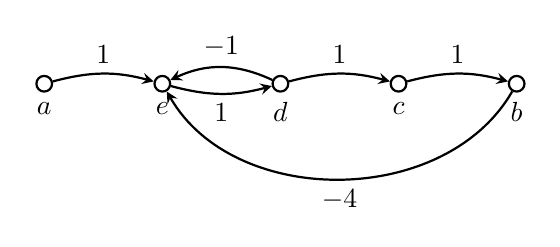
\begin{tikzpicture}
      [nodedecorate/.style={shape=circle,inner sep=2pt,draw,thick},%
      arrowdecorate/.style={->,>=stealth,thick}]
      %% nodes or vertices
      
      \foreach \nodename/\x/\y/\direction/\navigate in { a/0/0/below/south,
        b/6/0/below/south, c/4.5/0/below/south, d/3/0/below/south, e/1.5/0/below/south}
      {
        \node (\nodename) at (\x,\y) [nodedecorate] {};
        \node [\direction] at (\nodename.\navigate) {$\nodename$};
      }
      %% edges or lines
      \path
      \foreach \startnode/\endnode/\direction/\angle/\weight in {
        a/e/above/15/1, d/e/above/-25/-1, e/d/below/-15/1,  d/c/above/15/1, c/b/above/15/1, b/e/below/60/-4}
      {
        (\startnode) edge[arrowdecorate,bend left=\angle] node[\direction] {$\weight$} (\endnode)
      };
      ;
    \end{tikzpicture}
    \caption{Граф с отрицателен цикъл}
  \end{subfigure}
  \quad
  \begin{subtable}[b]{0.5\textwidth}
    \begin{tabular}{|c|c|c|c|c|}
      \hline
      $\delta(a)$ & $\delta(b)$ & $\delta(c)$ & $\delta(d)$ & $\delta(e)$ \\
      \hline
      0 & $\infty$ & $\infty$ & $\infty$ & {\bf \framebox{1}}\\
      \hline
      \hline
      $\colon$ & \framebox{$\infty$} & $\infty$ & $\infty$ & 1\\
      $\colon$ & $\infty$ & \framebox{$\infty$} & $\infty$ & 1\\
      $\colon$ & $\infty$ & $\infty$ & {\bf \framebox{2}} & 1\\
      $\colon$ & $\infty$ & $\infty$ & 2 & \framebox{1}\\
      \hline\hline
      $\colon$ & \framebox{$\infty$} & $\infty$ & 2 & 1\\
      $\colon$ & $\infty$ & {\bf \framebox{3}} & 2 & 1\\
      $\colon$ & $\infty$ & 3 & \framebox{2} & 1\\
      $\colon$ & $\infty$ & $\infty$ & 2 & \framebox{1}\\
      \hline\hline
      $\colon$ & {\bf \framebox{4}} & 3 & 2 & 1\\
      $\colon$ & 4 & \framebox{3} & 2 & 1\\
      $\colon$ & 4 & 3 & \framebox{2} & 1\\
      $\colon$ & 4 & 3 & 2 & {\bf \framebox{0}}\\
      \hline\hline
    \end{tabular}
    \caption{Изпълнение на алгоритъма}
  \end{subtable}
  \caption{Алгоритъм на Белман-Форд върху ориентиран граф с отрицателен цикъл,
  като ребрата са подредени лексикографски: $\pair{a,e}, \pair{b,e}, \pair{c,b}, \pair{d,c}, \pair{d,e}, \pair{e, d}$}
  \label{fig:bellman-ford-negative-cycle}
\end{figure}


\begin{figure}[!htbp]
  
\begin{subfigure}[b]{0.3\textwidth}
    \begin{tikzpicture}[scale=0.9]
      %% nodes or vertices
      
      \foreach \nodename/\value/\x/\y/\direction/\navigate/\color in { 
        s/0/0/0/left/west/green, 
        x/\infty/3.5/1.5/above/north/black,
        y/\infty/1/-1.5/below/south/black,
        t/\infty/1/1.5/above/north/black, 
        z/\infty/3.5/-1.5/below/south/black}
      {
        \node[vertex, nodedecorate, fill=\color!25] (\nodename) at (\x,\y) {$\value$};
        \node [\direction] at (\nodename.\navigate) {$\nodename$};
      }
      % edges or lines
      \path
      \foreach \startnode/\endnode/\direction/\angle/\weight in {
        s/t/left/15/6, s/y/left/-25/7, y/z/below/0/9,  t/y/left/0/8, t/x/above/30/5, x/t/above/30/-2, z/x/right/0/7,
        z/s/below/0/2, y/x/below/-3, t/z/right/15/-4
      }
      {
        (\startnode) edge[arrowdecorate,bend left=\angle] node[\direction] {$\weight$} (\endnode)
      };
      ;
    \end{tikzpicture}
    \caption{Начален връх е $s$}
  \end{subfigure}
  \quad
  \begin{subfigure}[b]{0.3\textwidth}
    \begin{tikzpicture}[scale=0.9]
      \foreach \nodename/\value/\x/\y/\direction/\navigate/\color in { 
        s/0/0/0/left/west/green, 
        x/\infty/3.5/1.5/above/north/black,
        y/7/1/-1.5/below/south/red,
        t/6/1/1.5/above/north/red, 
        z/\infty/3.5/-1.5/below/south/black}
      {
        \node[vertex, nodedecorate, fill=\color!25] (\nodename) at (\x,\y) {$\value$};
        \node [\direction] at (\nodename.\navigate) {$\nodename$};
      }
    
    \path
    \foreach \startnode/\endnode/\angle in {
      s/t/15, s/y/-25}
    {
      (\startnode) edge[selected edge, bend left=\angle] node[] {} (\endnode)
    };
    
    %edges
    \path
    \foreach \startnode/\endnode/\direction/\angle/\weight in {
      s/t/left/15/6, s/y/left/-25/7, y/z/below/0/9,  t/y/left/0/8, t/x/above/30/5, x/t/above/30/-2, z/x/right/0/7,
      z/s/below/0/2, y/x/below/-3, t/z/right/15/-4}
    {
      (\startnode) edge[arrowdecorate,bend left=\angle] node[\direction] {$\weight$} (\endnode)
    };
    

  \end{tikzpicture}
  \caption{Започваме със съседите на $s$}
  \end{subfigure}
  \quad
  \begin{subfigure}[b]{0.3\textwidth}
    \begin{tikzpicture}[scale=0.9]
      
      \foreach \nodename/\value/\x/\y/\direction/\navigate/\color in { 
        s/0/0/0/left/west/green, 
        x/4/3.5/1.5/above/north/red,
        y/7/1/-1.5/below/south/blue,
        t/6/1/1.5/above/north/blue, 
        z/2/3.5/-1.5/below/south/red}
      {
        \node[vertex, nodedecorate, fill=\color!25] (\nodename) at (\x,\y) {$\value$};
        \node [\direction] at (\nodename.\navigate) {$\nodename$};
      }
    
    \path
    \foreach \startnode/\endnode/\angle in {
      s/t/15, s/y/-25}
    {
      (\startnode) edge[path edge, bend left=\angle] node[] {} (\endnode)
    };


    %edges or lines
    \path
      (y) edge[selected edge] node[below] {} (x)
      (t) edge[selected edge, bend left=15] node[left] {} (z);

    \path
    \foreach \startnode/\endnode/\direction/\angle/\weight in {
      s/t/left/15/6, s/y/left/-25/7, y/z/below/0/9,  t/y/left/0/8, t/x/above/30/5, x/t/above/30/-2, z/x/right/0/7,
      z/s/below/0/2, y/x/below/0/-3, t/z/right/15/-4
    }
    {
      (\startnode) edge[arrowdecorate,bend left=\angle] node[\direction] {$\weight$} (\endnode)
    };
    ;

  \end{tikzpicture}
  \caption{Продължаваме с $x$ и $z$}
  \end{subfigure}
\quad
\begin{subfigure}[b]{0.3\textwidth}
  \begin{tikzpicture}[scale=0.9]
    
    \foreach \nodename/\value/\x/\y/\direction/\navigate/\color in { 
      s/0/0/0/left/west/green, 
      x/4/3.5/1.5/above/north/blue,
      y/7/1/-1.5/below/south/blue,
      t/2/1/1.5/above/north/red, 
      z/2/3.5/-1.5/below/south/blue}
    {
      \node[vertex, nodedecorate, fill=\color!25] (\nodename) at (\x,\y) {$\value$};
      \node [\direction] at (\nodename.\navigate) {$\nodename$};
    }
    
    \path
    \foreach \startnode/\endnode/\angle in {
      s/y/-25, y/x/0, t/z/15}
    {
      (\startnode) edge[path edge, bend left=\angle] node[] {} (\endnode)
    };

    \path
    \foreach \startnode/\endnode/\angle in {
      x/t/30
    }
    {
      (\startnode) edge[selected edge,bend left=\angle] node[] {} (\endnode)
    };
    %edges or lines
    \path
    \foreach \startnode/\endnode/\direction/\angle/\weight in {
      s/t/left/15/6, s/y/left/-25/7, y/z/below/0/9,  t/y/left/0/8, t/x/above/30/5, x/t/above/30/-2, z/x/right/0/7,
      z/s/below/0/2, y/x/below/0/-3, t/z/right/15/-4
    }
    {
      (\startnode) edge[arrowdecorate,bend left=\angle] node[\direction] {$\weight$} (\endnode)
    };
    ;
  \end{tikzpicture}
  \caption{По-кратък път до $t$}
\end{subfigure}
\quad
\begin{subfigure}[b]{0.3\textwidth}
  \begin{tikzpicture}[scale=0.9]
    %% nodes or vertices
    \foreach \nodename/\value/\x/\y/\direction/\navigate/\color in { 
      s/0/0/0/left/west/green, 
      x/4/3.5/1.5/above/north/blue,
      y/7/1/-1.5/below/south/blue,
      t/2/1/1.5/above/north/blue, 
      z/-2/3.5/-1.5/below/south/red}
    {
      \node[vertex, nodedecorate, fill=\color!25] (\nodename) at (\x,\y) {$\value$};
      \node [\direction] at (\nodename.\navigate) {$\nodename$};
    }
    \path
    \foreach \startnode/\endnode/\angle in {
      s/y/-25, y/x/0, x/t/30}
    {
      (\startnode) edge[path edge, bend left=\angle] node[] {} (\endnode)
    };
    \path
    \foreach \startnode/\endnode/\angle in {
      t/z/15/
    }
    {
      (\startnode) edge[selected edge,bend left=\angle] node[] {} (\endnode)
    };
    %edges or lines
    \path
    \foreach \startnode/\endnode/\direction/\angle/\weight in {
      s/t/left/15/6, s/y/left/-25/7, y/z/below/0/9,  t/y/left/0/8, t/x/above/30/5, x/t/above/30/-2, z/x/right/0/7,
      z/s/below/0/2, y/x/below/0/-3, t/z/right/15/-4
    }
    {
      (\startnode) edge[arrowdecorate,bend left=\angle] node[\direction] {$\weight$} (\endnode)
    };
  \end{tikzpicture}
  \caption{По-кратък път до $z$}
  \end{subfigure}
\quad
\begin{subfigure}[b]{0.3\textwidth}
  \begin{tikzpicture}[scale=0.9]
    %% nodes or vertices
    \foreach \nodename/\value/\x/\y/\direction/\navigate/\color in { 
      s/0/0/0/left/west/green, 
      x/4/3.5/1.5/above/north/blue,
      y/7/1/-1.5/below/south/blue,
      t/2/1/1.5/above/north/blue, 
      z/-2/3.5/-1.5/below/south/blue}
    {
      \node[vertex, nodedecorate, fill=\color!25] (\nodename) at (\x,\y) {$\value$};
      \node [\direction] at (\nodename.\navigate) {$\nodename$};
    }
    \path
    \foreach \startnode/\endnode/\angle in {
      s/y/-25, y/x/0, x/t/30, t/z/15}
    {
      (\startnode) edge[path edge, bend left=\angle] node[] {} (\endnode)
    };
    %edges or lines
    \path
    \foreach \startnode/\endnode/\direction/\angle/\weight in {
      s/t/left/15/6, s/y/left/-25/7, y/z/below/0/9,  t/y/left/0/8, t/x/above/30/5, x/t/above/30/-2, z/x/right/0/7,
      z/s/below/0/2, y/x/below/0/-3, t/z/right/15/-4
    }
    {
      (\startnode) edge[arrowdecorate,bend left=\angle] node[\direction] {$\weight$} (\endnode)
    };
  \end{tikzpicture}
  \caption{Край на процедурата.}
\end{subfigure}


%%% Local Variables: 
%%% mode: latex
%%% TeX-master: "discrete-math"
%%% End: 

  \index{Белман-Форд!алгоритъм}
  \caption{Алгоритъм на Белман-Форд запазващ минималните пътища}
  \label{fig:bellman-ford-graph}
\end{figure}


%% стр. 654
\begin{problem}
  Променете алгоритъма на Белман-Форд, така че $\delta(v) = -\infty$ за всеки връх $v$, 
  за който има отрицателен цикъл по някой път от началния връх $s$ до $v$.
\end{problem}



%%% Local Variables: 
%%% mode: latex
%%% TeX-master: "discrete-math"
%%% End: 
